\documentclass{article}

\usepackage[T1]{fontenc}
\usepackage[polish]{babel}
\usepackage{geometry}
\usepackage{graphicx}
\usepackage{amsmath}
\usepackage{algorithm}
\usepackage{algpseudocode}

\title{Projekt 2 - Eliminacja Gaussa i LU faktoryzacja}
\author{Cyprian Neugebauer}
\date{}

\begin{document}
\maketitle

\section{Eliminacja Gaussa}

\subsection{Pseudokod}

Algorytm eliminacji Gaussa można opisać następującymi krokami:

\begin{enumerate}
    \item Weź macierz $A$ i wektor $b$, gdzie $A$ jest macierzą współczynników układu równań, a $b$ jest wektorem wyrazów wolnych.
    \item Dołącz wektor $b$ do macierzy $A$ jako dodatkową kolumnę, tworząc rozszerzoną macierz $Ab$.
    \item Dla każdego wiersza $i$ od $1$ do $n$ (gdzie $n$ jest liczbą wierszy macierzy $A$):
    \begin{enumerate}
        \item Normalizuj wiersz $i$ przez podzielenie go przez element diagonalny $Ab_{i,i}$, aby na przekątnej uzyskać $1$.
        \item Dla każdego wiersza $j$ poniżej $i$ (od $i+1$ do $n$):
        \begin{enumerate}
            \item Odejmij od wiersza $j$ wiersz $i$ pomnożony przez $Ab_{j,i}$, aby wyzerować elementy poniżej przekątnej w kolumnie $i$.
        \end{enumerate}
    \end{enumerate}
    \item Inicjalizuj wektor rozwiązań $x$ o długości $n$.
    \item Rozwiąż układ równań od ostatniego wiersza do pierwszego:
    \begin{enumerate}
        \item Dla każdego wiersza $i$ od $n$ do $1$, oblicz $x_i = Ab_{i,n+1} - \sum_{k=i+1}^{n} Ab_{i,k} \cdot x_k$.
    \end{enumerate}
    \item Zwróć wektor rozwiązań $x$.
\end{enumerate}

\begin{algorithm}[H]
\caption{Gaussian Elimination}
\begin{algorithmic}[1]
\Procedure{GaussianElimination}{$A, b$}
    \State $n \gets \text{rows}(A)$
    \State $Ab \gets \text{concatenate}(A, b, \text{axis}=1)$
    \\
    \For{$i \gets 0$ \textbf{to} $n-1$}
        \State $Ab[i, i:] \gets Ab[i, i:] / Ab[i, i]$
        \For{$j \gets i+1$ \textbf{to} $n-1$}
            \State $Ab[j, i:] \gets Ab[j, i:] - Ab[j, i] \cdot Ab[i, i:]$
        \EndFor
    \EndFor
    \\
    \State $x \gets \text{zeroes}(n)$
    \For{$i \gets n-1$ \textbf{down to} $0$}
        \State $x[i] \gets Ab[i, n] - Ab[i, i+1 : n] \cdot x[i+1 :]$
    \EndFor
    \\
    \State \textbf{return} $x$
\EndProcedure
\end{algorithmic}
\end{algorithm}

\subsection{Kod algorytmu}

\begin{figure}[htbp]
  \centering
  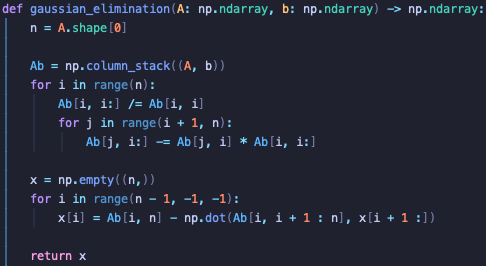
\includegraphics[width=0.9\linewidth]{gaussian_elimination.png}
  \caption{Kod eliminacji Gaussa}
  \label{fig:gaussian_elimination}
\end{figure}

\subsection{Porównanie wyników}

\begin{figure}[htbp]
  \centering
  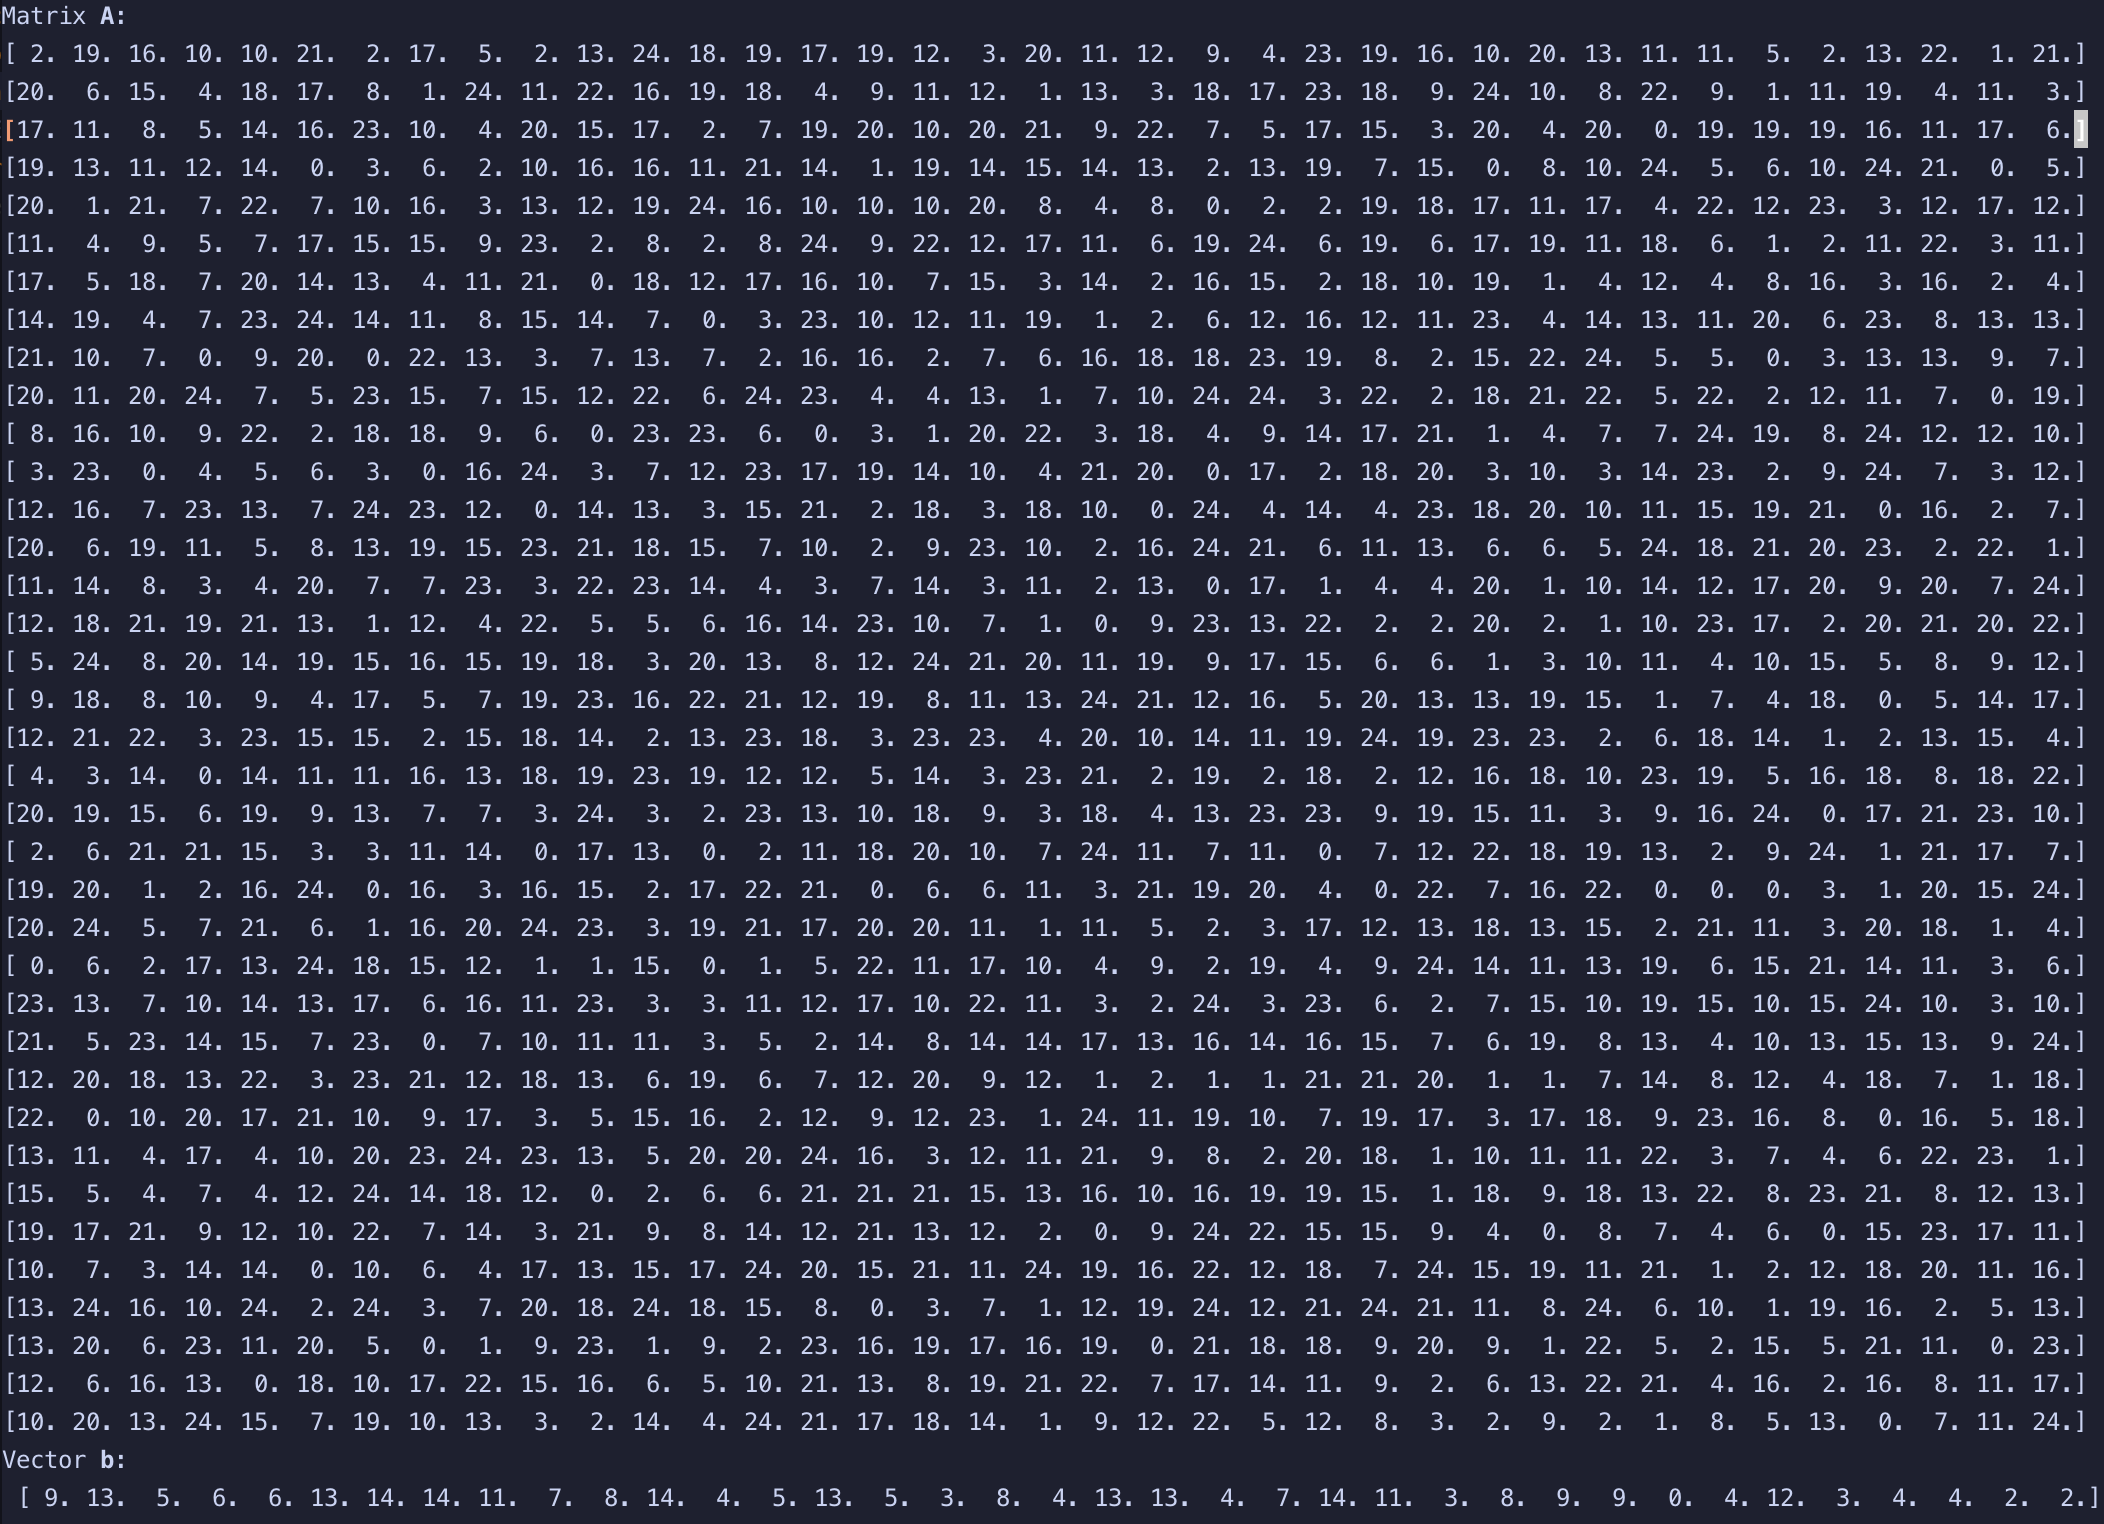
\includegraphics[width=0.9\linewidth]{Ab.png}
  \caption{Wylosowana macierz gęsta $A_{37x37}$ i wektor $\textbf{b}$}
  \label{fig:Ab}
\end{figure}

\begin{figure}[H]
  \centering
  \begin{minipage}[b]{0.45\linewidth}
    \centering
    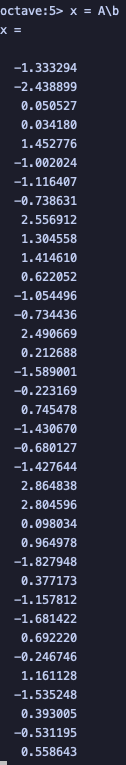
\includegraphics[height=10cm]{x_matlab.png}
    \caption{Rozwiązanie $x$ obliczone w programie MATLAB}
    \label{fig:x_matlab}
  \end{minipage}
  \begin{minipage}[b]{0.45\linewidth}
    \centering
    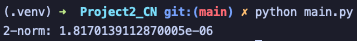
\includegraphics[width=\linewidth]{2norm1.png}
    \caption{Wartość normy $L_2$ dla różnicy rozwiązania w MATLAB z własnym rozwiązaniem eliminacją Gaussa bez pivotingu}
    \label{fig:2norm1}
  \end{minipage}
\end{figure}

Wartość normy wynosząca $~ 1.8 \times 10^{-6}$ jest bardzo bliska zeru, co oznacza, że rozwiązania są identyczne, a norma nie jest równa 0 przez skończoną precyzję zapisu liczb zmiennoprzecinkowych.

\section{Eliminacja Gaussa z pivotingiem}

\subsection{Pseudokod}

Algorytm eliminacji Gaussa z częściowym wyborem pivota można opisać następującymi krokami:

\begin{enumerate}
    \item Weź macierz $A$ i wektor $b$, gdzie $A$ jest macierzą współczynników układu równań, a $b$ jest wektorem wyrazów wolnych.
    \item Dołącz wektor $b$ do macierzy $A$ jako dodatkową kolumnę, tworząc rozszerzoną macierz $Ab$.
    \item Dla każdego wiersza $i$ od $1$ do $n$ (gdzie $n$ jest liczbą wierszy macierzy $A$):
    \begin{enumerate}
        \item Znajdź wiersz $p$ poniżej wiersza $i$ (włącznie z $i$), który ma największą wartość bezwzględną elementu w kolumnie $i$. Wiersz ten staje się nowym wierszem pivota.
        \item Zamień wiersz $i$ z wierszem pivota $p$.
        \item Normalizuj wiersz $i$ przez podzielenie go przez element diagonalny $Ab_{i,i}$, aby na przekątnej uzyskać $1$.
        \item Dla każdego wiersza $j$ poniżej $i$ (od $i+1$ do $n$):
        \begin{enumerate}
            \item Odejmij od wiersza $j$ wiersz $i$ pomnożony przez $Ab_{j,i}$, aby wyzerować elementy poniżej przekątnej w kolumnie $i$.
        \end{enumerate}
    \end{enumerate}
    \item Inicjalizuj wektor rozwiązań $x$ o długości $n$.
    \item Rozwiąż układ równań od ostatniego wiersza do pierwszego:
    \begin{enumerate}
        \item Dla każdego wiersza $i$ od $n$ do $1$, oblicz $x_i = Ab_{i,n+1} - \sum_{k=i+1}^{n} Ab_{i,k} \cdot x_k$.
    \end{enumerate}
    \item Zwróć wektor rozwiązań $x$.
\end{enumerate}

\begin{algorithm}
\caption{Pivot Gaussian Elimination}
\begin{algorithmic}[1]
\Procedure{PivotGaussianElimination}{$A, b$}
    \State $n \gets \text{rows}(A)$
    \State $Ab \gets \text{concatenate}(A, b, \text{axis}=1)$
    \\
    \For{$i \gets 0$ \textbf{to} $n-1$}
        \State $pivot \gets i + \text{argmax}(\text{abs}(Ab[i:, i]))$
        \State $Ab[i, i:] \gets Ab[i, i:] / Ab[i, i]$
        \For{$j \gets i+1$ \textbf{to} $n-1$}
            \State $Ab[j, i:] \gets Ab[j, i:] - Ab[j, i] \cdot Ab[i, i:]$
        \EndFor
    \EndFor
    \\
    \State $x \gets \text{empty vector of length } n$
    \For{$i \gets n-1$ \textbf{down to} $0$}
        \State $x[i] \gets Ab[i, n] - Ab[i, i+1 : n] \cdot x[i+1 :]$
    \EndFor
    \\
    \State \textbf{return} $x$
\EndProcedure
\end{algorithmic}
\end{algorithm}

\subsection{Kod algorytmu}

\begin{figure}[H]
  \centering
  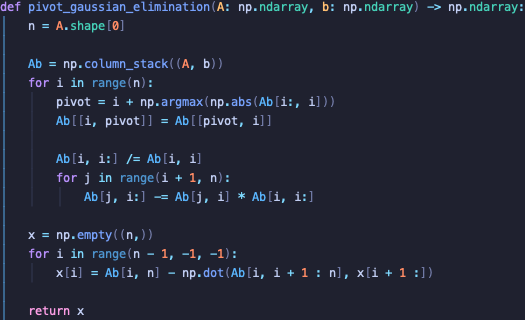
\includegraphics[width=0.9\linewidth]{pivot_gaussian_elimination.png}
  \caption{Kod eliminacji Gaussa z pivotingiem}
  \label{fig:pivot_gaussian_elimination}
\end{figure}

\subsection{Porównanie wyników}

\begin{figure}[H]
    \centering
    
\includegraphics[width=\linewidth]{2norm2.png}
    \caption{Wartość normy $L_2$ dla różnicy rozwiązania w MATLAB z własnym rozwiązaniem eliminacją Gaussa z pivotingiem}
    \label{fig:2norm2}
\end{figure}

Dla eliminacji Gaussa z pivotingiem występuje taka sama sytuacja jak bez pivotingu. Otrzymane rozwiązania są identyczne z MATLAB.

\section{LU faktoryzacja}

\subsection{Pseudokod}

Algorytm dekompozycji LU dla macierzy $A$ można opisać następującymi krokami:

\begin{enumerate}
    \item Weź kwadratową macierz $A$ o wymiarach $n \times n$.
    \item Inicjalizuj macierz $L$ jako macierz jednostkową rozmiaru $n \times n$ i macierz $U$ jako kopię macierzy $A$.
    \item Dla każdego wiersza $i$ od $1$ do $n$ wykonaj:
    \begin{enumerate}
        \item Dla każdego wiersza $j$ od $i+1$ do $n$ wykonaj:
        \begin{enumerate}
            \item Oblicz współczynnik $L_{j,i} = U_{j,i} / U_{i,i}$ i zapisz go w macierzy $L$ na pozycji $(j,i)$.
            \item Zaktualizuj wiersz $j$ w macierzy $U$ poprzez odjęcie $L_{j,i}$ razy wiersz $i$ w macierzy $U$, zaczynając od kolumny $i$. Czyli wykonaj operację $U_{j,i:} -= L_{j,i} \cdot U_{i,i:}$.
        \end{enumerate}
    \end{enumerate}
    \item Zwróć macierz $L$ i macierz $U$ jako wynik dekompozycji LU.
\end{enumerate}

\begin{algorithm}
\caption{LU Decomposition}
\begin{algorithmic}[1]
\Procedure{LUDecomposition}{$A$}
    \State $n \gets \text{rows}(A)$
    \State $L \gets \text{eye}(n)$
    \State $U \gets A.\text{copy}()$
    \\
    \For{$i \gets 0$ \textbf{to} $n-1$}
        \For{$j \gets i+1$ \textbf{to} $n-1$}
            \State $L[j, i] \gets U[j, i] / U[i, i]$
            \State $U[j, i:] \gets U[j, i:] - L[j, i] \cdot U[i, i:]$
        \EndFor
    \EndFor
    \\
    \State \textbf{return} $L, U$
\EndProcedure
\end{algorithmic}
\end{algorithm}

\subsection{Kod algorytmu}

\begin{figure}[htbp]
  \centering
  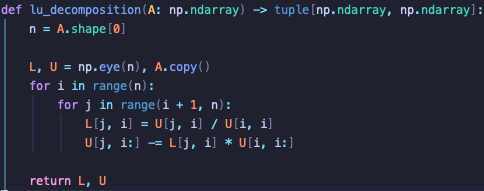
\includegraphics[width=0.9\linewidth]{lu.png}
  \caption{Kod faktoryzacji LU}
  \label{fig:lu}
\end{figure}

\subsection{Porównanie wyników}

\begin{figure}[htbp]
  \centering
  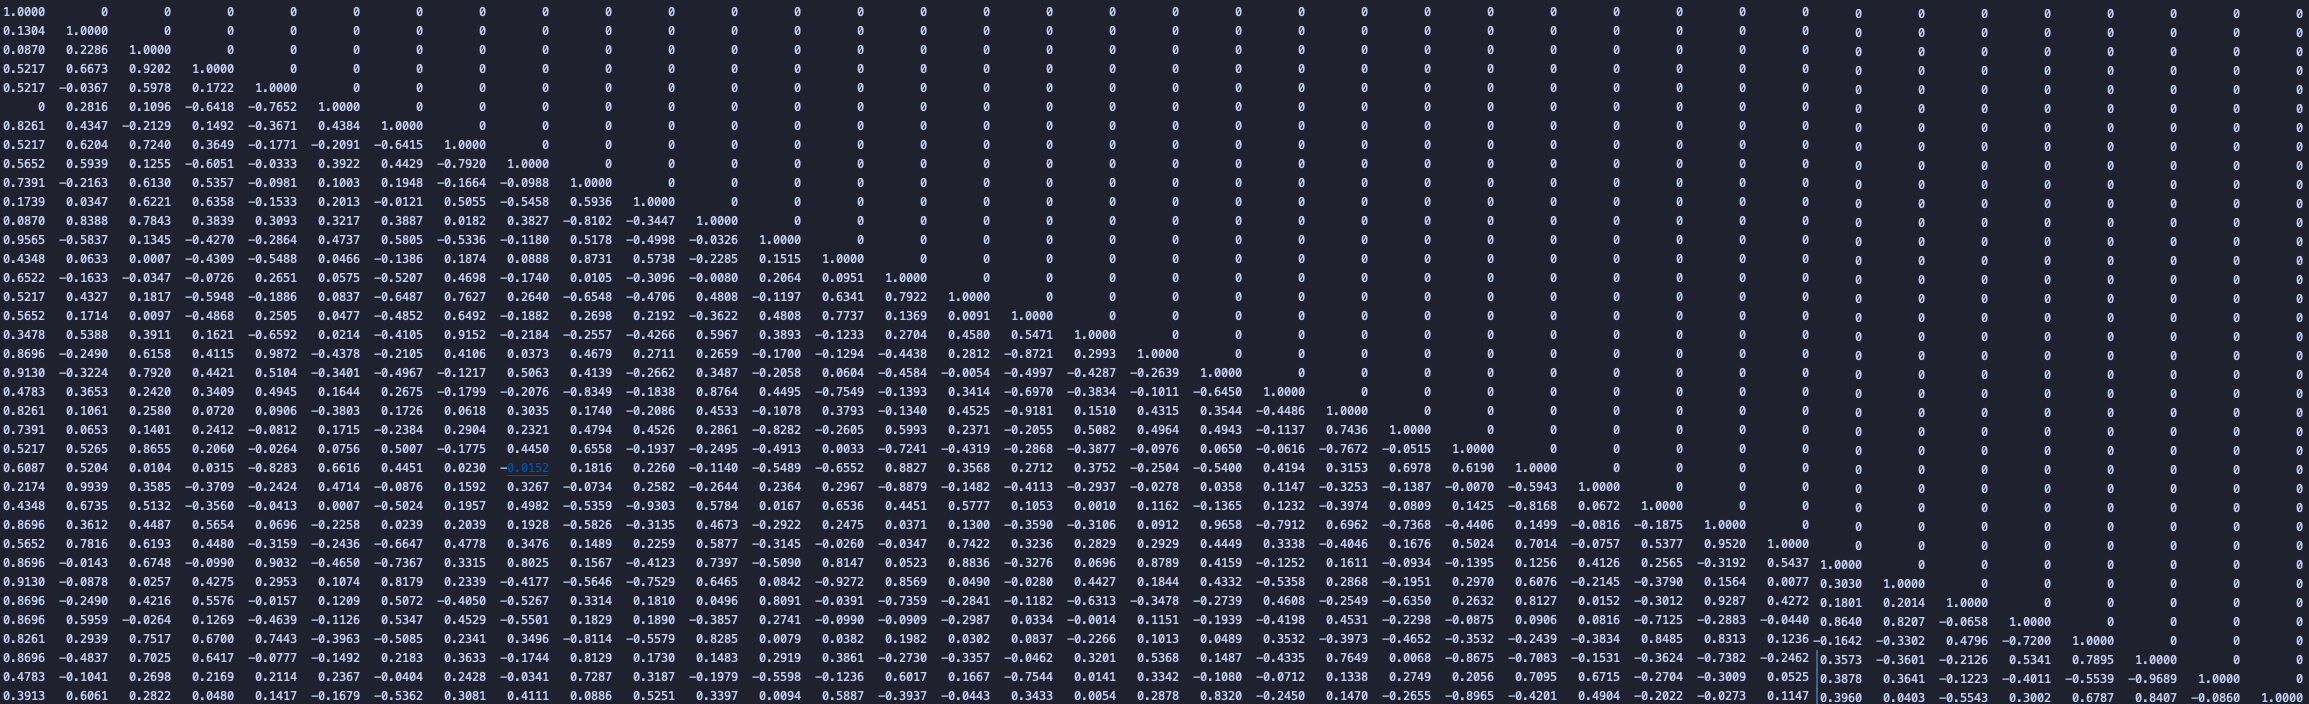
\includegraphics[width=\linewidth]{l_matlab.png}
  \caption{Macierz L faktoryzacji LU z MATLAB}
  \label{fig:l_matlab}
\end{figure}

\begin{figure}[htbp]
  \centering
  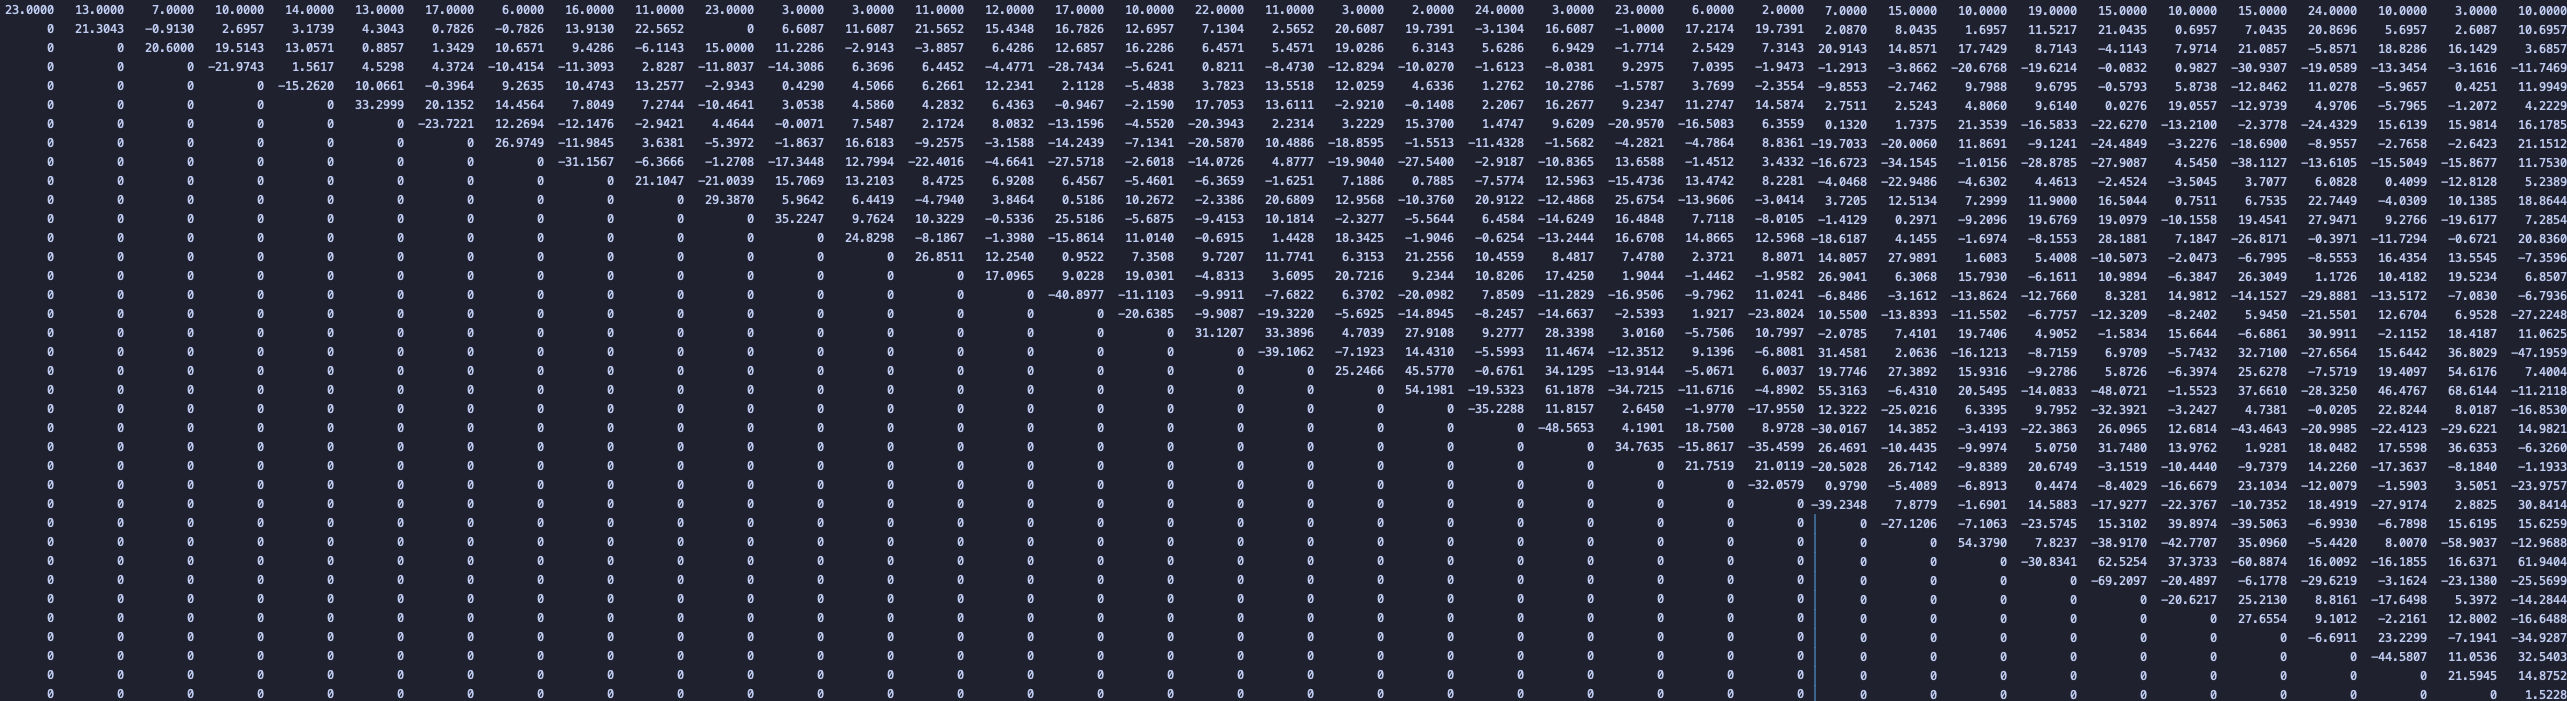
\includegraphics[width=\linewidth]{u_matlab.png}
  \caption{Macierz U faktoryzacji LU z MATLAB}
  \label{fig:u_matlab}
\end{figure}

\begin{figure}[H]
  \centering
  
\includegraphics[width=\linewidth]{p_matlab.png}
  \caption{Macierz permutacji P faktoryzacji LU z MATLAB}
  \label{fig:p_matlab}
\end{figure}

\begin{figure}[htbp]
  \centering
  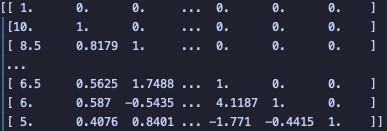
\includegraphics[width=\linewidth]{l_python1.png}
  \caption{Macierz L faktoryzacji LU z własnego rozwiązania}
  \label{fig:l_python1}
\end{figure}

\begin{figure}[H]
  \centering
  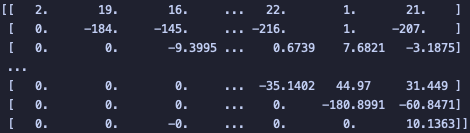
\includegraphics[width=\linewidth]{u_python1.png}
  \caption{Macierz U faktoryzacji LU z własnego rozwiązania}
  \label{fig:u_python1}
\end{figure}

Macierze L i U zwrócone z MATLAB różnią się od L i U zwróconych z własnego rozwiązania. Wynika to z faktu, że MATLAB używa częściowego wyboru pivota, co wpływa na wynik dekompozycji LU. Własne rozwiązanie nie używa pivotingu, więc wyniki mogą się różnić.

\section{LU faktoryzacja z pivotingiem}

\subsection{Pseudokod}

Algorytm dekompozycji LU z częściowym wyborem pivota dla macierzy $A$ można opisać następującymi krokami:

\begin{enumerate}
    \item Weź kwadratową macierz $A$ o wymiarach $n \times n$.
    \item Inicjalizuj wektor permutacji $perm$ jako ciąg liczb od $0$ do $n-1$, macierz $L$ jako macierz jednostkową rozmiaru $n \times n$ i macierz $U$ jako kopię macierzy $A$.
    \item Dla każdego wiersza $i$ od $1$ do $n$ wykonaj:
    \begin{enumerate}
        \item Znajdź indeks $pivot$ największego (w wartości bezwzględnej) elementu w kolumnie $i$ wierszy od $i$ do $n$.
        \item Zamień wiersze $i$ i $pivot$ w macierzy $L$, w kolumnach od $1$ do $i-1$.
        \item Zamień wiersze $i$ i $pivot$ w macierzy $U$.
        \item Zamień elementy $i$ i $pivot$ w wektorze permutacji $perm$.
        \item Dla każdego wiersza $j$ od $i+1$ do $n$ wykonaj:
        \begin{enumerate}
            \item Oblicz współczynnik $L_{j,i} = U_{j,i} / U_{i,i}$ i zapisz go w macierzy $L$ na pozycji $(j,i)$.
            \item Zaktualizuj wiersz $j$ w macierzy $U$ poprzez odjęcie $L_{j,i}$ razy wiersz $i$ w macierzy $U$, zaczynając od kolumny $i$. Czyli wykonaj operację $U_{j,i:} -= L_{j,i} \cdot U_{i,i:}$.
        \end{enumerate}
    \end{enumerate}
    \item Inicjalizuj wektor odwrotnej permutacji $inv\_perm$ i dla każdego indeksu w $perm$ zapisz odwrotną permutację.
    \item Zastosuj odwrotną permutację do wierszy macierzy $L$.
    \item Zwróć macierz $L$ i macierz $U$ jako wynik dekompozycji LU.
\end{enumerate}

\begin{algorithm}
\caption{Pivot LU Decomposition}
\begin{algorithmic}[1]
\Procedure{PivotLUDecomposition}{$A$}
    \State $n \gets \text{rows}(A)$
    \State $perm \gets \text{range}(n)$
    \State $L \gets \text{eye}(n)$
    \State $U \gets A.\text{copy}()$
    \\
    \For{$i \gets 0$ \textbf{to} $n-1$}
        \State $pivot \gets i + \text{argmax}(\text{abs}(U[i:, i]))$
        \State Swap $L[i, :i]$ and $L[pivot, :i]$
        \State Swap $U[i, :]$ and $U[pivot, :]$
        \State Swap $perm[i]$ and $perm[pivot]$
        \\
        \For{$j \gets i+1$ \textbf{to} $n-1$}
            \State $L[j, i] \gets U[j, i] / U[i, i]$
            \State $U[j, i:] \gets U[j, i:] - L[j, i] \cdot U[i, i:]$
        \EndFor
    \EndFor
    \\
    \State $inv\_perm \gets \text{empty}(n, \text{dtype}=\text{int})$
    \State $inv\_perm[perm] \gets \text{range}(n)$
    \\
    \State \textbf{return} $L[inv\_perm], U$
\EndProcedure
\end{algorithmic}
\end{algorithm}

\subsection{Kod algorytmu}

\begin{figure}[htbp]
  \centering
  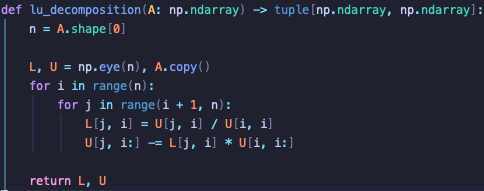
\includegraphics[width=0.9\linewidth]{lu.png}
  \caption{Kod faktoryzacji LU z pivotingiem}
  \label{fig:pivot_lu}
\end{figure}

\subsection{Porównanie wyników}

\begin{figure}[htbp]
  \centering
  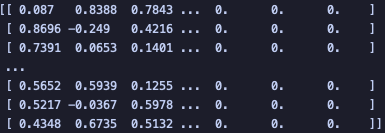
\includegraphics[width=\linewidth]{l_python2.png}
  \caption{Macierz L faktoryzacji LU z własnego rozwiązania}
  \label{fig:l_python2}
\end{figure}

\begin{figure}[H]
  \centering
  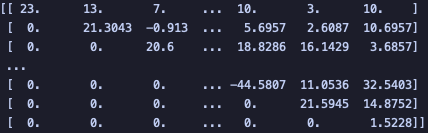
\includegraphics[width=\linewidth]{u_python2.png}
  \caption{Macierz U faktoryzacji LU z własnego rozwiązania}
  \label{fig:u_python2}
\end{figure}

Macierz L zwrócona z własnego programu różni się od macierzy L zwróconej z MATLAB, natomiast jest to spowodowane tym, że w moim programie stosuję od razu odwrotną permutację, podczas gdy MATLAB zwraca macierz L z permutacją. Macierze U zwrócone z obu programów są identyczne.

\end{document}
